% !TeX spellcheck = ru_RU
% !TEX root = vkr.tex

\section{Подробности реализации}

В силу требования гомогенности, удобства работы с древовидными типами данных, естественно возникающими в компиляторах, и наличия языка описания аппаратуры Clash\footnote{Сайт проекта: \url{https://clash-lang.org/} (дата обращения \DTMdate{2025-05-18})}, используемого в блоке Hardware, в качестве языка реализации проекта был выбран \Haskell{}.
Архитектура изображена на рисунке~\ref{fig:lmlcmods}.

Для сборки проекта и версионирования зависимостей используется \textsc{Stack}\footnote{Сайт проекта: \url{https://docs.haskellstack.org/en/stable/} (дата обращения \DTMdate{2025-02-25})}, предоставляющий снимки репозитория пакетов с гарантированно совместимыми пакетами.
Для тестирования используется фреймворк \textsc{Tasty}\footnote{Описание проекта на \textsc{Hackage}: \url{https://hackage.haskell.org/package/tasty/} (дата обращения \DTMdate{2025-02-25})}, позволяющий через единый интерфейс писать и запускать различные виды тестов: модульные, golden, property-based.
Поскольку тестирование трансляторов с помощью модульных тестов довольно сложно, по умолчанию все части компилятора покрываются интеграционными golden\footnote{Описание golden тестов: \url{https://ro-che.info/articles/2017-12-04-golden-tests} (дата обращения \DTMdate{2025-02-25})} тестами.

\begin{figure}[h]
    \begin{center}
        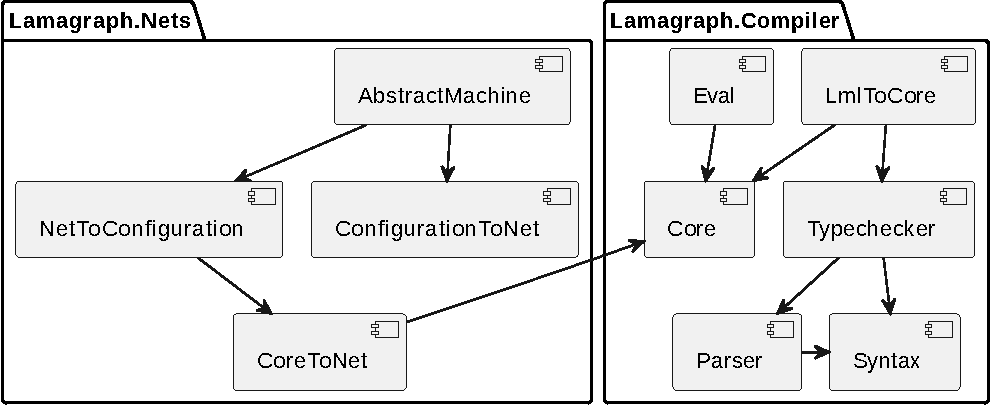
\includegraphics[width=0.8\linewidth]{components}
    \end{center}
    \caption{Архитектура транслятора}
    \label{fig:lmlcmods}
\end{figure}

\paragraph{Синтаксис языка.}

Синтаксис языка основан на \OCaml{}.
Однако упрощен для простоты реализации\footnote{С полной грамматикой можно ознакомиться в репозитории проекта: \url{https://github.com/Lamagraph/interaction-nets-in-fpga/blob/main/lamagraph-compiler/src/Lamagraph/Compiler/Syntax.hs} (дата обращения \DTMdate{2025-02-25})}.
Так, например, в языке остались стандартные для функциональных языков конструкции, такие как сопоставление с образцом, рекурсивные и взаимнорекурсивные функции, а также алгебраические типы данных.
В отличие от \OCaml{} отсутствует поддержка классов и функторов, а система модулей максимально упрощена и напоминает систему модулей в F\#.

Для представления AST (дерева абстрактного синтаксиса) используется паттерн Trees That Grow (TTG)~\cite{shayannajdTreesThatGrow}.
Он позволяет с помощью механизма type families~\cite{schrijversTypeCheckingOpen2008} гибко параметризовать дерево необходимыми аннотациями, более того аннотации могут различаться в разных узлах дерева, тем самым поддерживая безопасность кода.

\paragraph{Парсер.}

Для синтаксического анализа используется стандартная для \Haskell{} связка лексера \textsc{Alex} и парсер-генератора \textsc{Happy}, которые являются аналогами \textsc{flex} и \textsc{bison} и используются в крупных проектах, например GHC.

На данном этапе работы транслятора аннотации с помощью TTG не используются.

Для тестирования лексера используются модульные тесты.
Для парсера используется property-based тестирование с использованием библиотеки \textsc{Hedgehog}\footnote{Репозиторий проекта: \url{https://github.com/hedgehogqa/haskell-hedgehog/} (дата обращения: \DTMdate{2025-02-19})}.
Данный метод основан на том, что синтаксический анализ в AST и печать AST должны давать тождественное отображение при композиции.

\paragraph{Вывод типов.}

Поскольку язык ML-подобный, используется система типов Хиндли-Милнера~\cite{hindleyPrincipalTypeSchemeObject1969, milnerTheoryTypePolymorphism1978}.

После вывода типов в аннотациях TTG сохраняется тип каждого узла дерева.

В силу ограниченности времени, на данном этапе отсутствует поддержка пользовательских алгебраических типов данных.
Тем не менее поддержка типов \texttt{list} и \texttt{option} присутствует.

\paragraph{Промежуточное представление.}

AST, получаемое после синтаксического анализа и вывода типов, содержит большое количество различных типов узлов с аннотациями.
Для дальнейшей обработки используется упрощенное представление на основе GHC Core\footnote{Подробнее можно прочитать по ссылке: \url{https://gitlab.haskell.org/ghc/ghc/-/wikis/commentary/compiler/core-syn-type} (дата обращения: \DTMdate{2025-02-19})}, также часто называемое обогащённым $\lambda$-исчислением\footnote{Подробнее узнать про способы обогащения $\lambda$-исчисления можно в~\cite[раздел~3.2]{peytonjones1987the}}.
Его описание представлено на листинге~\ref{lst:core}.

\begin{listing}
    \inputminted[fontsize=\footnotesize]{haskell}{figures/core.hs}
    \caption{Представление Core в алгебраических типах данных.}
    \label{lst:core}
\end{listing}

Представление, используемое в данной работе, отличается от GHC Core наличием выделенного конструктора для пар, а также отсутствием типизации.

Наличие выделенного конструктора для пар обусловлено различием между ML и \Haskell{}~--- в первом пары тоже выделены и могут быть какой угодно арности, во втором же пара является синтаксическим сахаром для алгебраического типа-суммы и ограничена арностью 63.

От типизации пришлось отказаться в угоду простоты реализации, а также в виду отсутствия оптимизаций со стороны компилятора, где наличие типов упрощает и делает более безопасным их применение.

\paragraph{Трансляция высокоуровневого AST в промежуточное представление.}

На данный момент алгоритм трансляции достаточно прямолинеен.
Связано это с тем, что в левой части let-связываний поддерживаются только простые шаблоны (переменные), а в match-выражениях не поддерживаются вложенные шаблоны, защитные выражения и ИЛИ-шаблоны.

\paragraph{Интерпретатор обогащенного $\lambda$-исчисления.}

Интерпретатор реализован на основе идей из~\cite{reynoldsDefinitionalInterpretersHigherorder1972}.
Для реализации функций высшего порядка используются замыкания, для рекурсивных let-связываний используется \enquote{ленивость} \Haskell{} для создания рекурсивных замыканий, остальная часть работы интерпретатора довольно прямолинейна.

В текущей реализации интерпретатор наследует порядок исполнения от языка, на котором написан, в случае \Haskell{}~--- это call-by-need.
Это можно исправить с помощью продолжений (continuations), однако поскольку схема трансляции и порядок исполнения \INs{} по умолчанию не определен, на данном этапе было решено оставить call-by-need.

Кроме того, на данный момент отсутствует поддержка взаимной рекурсии.

\paragraph{Интерпретатор \INs{}.}

Стандартным представлением для \INs{} является графовое.
Однако для представления графов в функциональных языках не удаётся использовать их возможности по работе с алгебраическими типами данных и сопоставлением с образцом\footnote{Алгебраические графы, описанные в \cite{mokhovAlgebraicGraphsClass2017}, позволяют использовать сопоставление с образцом для обработки графов. Однако неизвестно, можно ли выразить все особенности \INs{} с помощью данной кодировки (например, упорядоченность дополнительных портов), кроме того неизвестно насколько естественно выражаются необходимые для редукции трансформации.}, поэтому потребовалось найти альтернативное представление.
Таковым стало текстовое представление Fernández и Mackie~\cite{fernandezCalculusInteractionNets1999}.
Для него также существует абстрактная машина~\cite{pintoSequentialConcurrentAbstract2000}, которая и была реализована.

\paragraph{Транслятор обогащенного $\lambda$-исчисления в \INs{}.}

Как было сказано в разделе~\ref{sec:ins}, существует не один способ трансляции $\lambda$-исчисления в \INs{}.
Поскольку мы транслируем ML-подобный язык, то первой схемой трансляции была выбрана схема call-by-value из~\cite{sinotCallbyNameCallbyValueTokenPassing2005}.
Для $\lambda$-абстракции и аппликации используются выделенные агенты, переменные же выражаются с помощью проводов.
В случае, если какая-то переменная используется более одного раза, используются агенты-дупликаторы.

В процессе реализации была обнаружена проблема: существующие схемы трансляции работают только с чистым $\lambda$-исчислением.
Попытки расширить схему трансляции предпринимались в~\cite{jireschExtendingInteractionNets2012}, однако такой подход требует использование динамического базиса агентов.
Но поскольку вычислитель прошивается на ПЛИС, то базис агентов должен быть фиксирован, и подход предложенный в статье нам не подходит.

Проблему можно попробовать решить на уровне $\lambda$-исчисления, используя кодировки Чёрча~\cite{barendregtImpactLambdaCalculus1997} или Скотта~\cite{koopmanChurchEncodingData2014}.
Однако скорее всего сети в таком случае будут получаться сложнее, чем могли бы, и будут требовать больше шагов редукции, кроме того такой подход отчасти противоречит параметризуемости \INs{}.
Поэтому трансляция в \INs{} конструкций обогащённого $\lambda$-исчисления~--- предмет дальнейшей работы.

Однако одну конструкцию обогащенного $\lambda$-исчисления, let-связывание, удалось  транслировать.
Для нерекурсивых связываний использовалась схема, похожая на схему работы с переменными; для рекурсивных, функция дополнительно применялась к комбинатору неподвижной точки.
